\documentclass[11pt]{article}
% guidelines at http://tab.computer.org/tcde/bull_author.html
\usepackage{deauthor,times,graphicx}
%\graphicspath{{authorname/}}

%\usepackage[dvipsnames,svgnames]{xcolor}
\usepackage{tikz}
\usepackage{amssymb, framed}
\usepackage{rotating}
\usepackage{xcolor}
\usepackage{hyperref}
\usepackage{tikz}
\usetikzlibrary{trees,shapes,snakes,patterns}
% % % --------------------------------------- % % %
% % % Macros to write comments for internal usage % % %
% % % --------------------------------------- % % %

\newcommand{\red}[1]{\textcolor{red}{#1}}

\begin{document}
\title{Platform Design for Crowdsourcing and Future of Work}
%The future of Crowdsourcing Platforms: Ecosystems and Interoperability}

\author{David\, Gross-Amblard\\
 University of Rennes, France\\
\texttt{{\footnotesize dga@irisa.fr}}
\and
Atsuyuki Morishima\\
University of Tsukuba\\
\texttt{{\footnotesize mori@slis.tsukuba.ac.jp}}
\and
Saravanan Thirumuruganathan\\
QCRI, HBKU\\
\texttt{{\footnotesize sthirumuruganathan@hbku.edu.qa}}
\and
Marion\, Tommasi\\
University of Lille and INRIA\\
\texttt{{\footnotesize marion.tommasi@inria.fr}}
\and
Ko\, Yoshida\\
CrowdWorks\\
\texttt{{\footnotesize yoshida@crowdworks.co.jp}}
}
\maketitle

\newcommand{\scream}[1]{\textbf{***#1***}}

% -------------------------------------------------------- %

\begin{abstract}
Online job platforms have proliferated in the last few years.
We anticipate a future where there exists thousands of such platforms covering wide swathes of tasks.
These include crowdsourcing platforms such as Amazon Mechanical Turk (AMT), CrowdWorks, Figure Eight;
specialized services such as ride-hailing;
matching markets such as TaskRabbit that matches workers with local demand and so on.
It is widely anticipated that a vast majority of human workforce will be employed in these platforms.
In this article, we initiate discussions about the under studied aspect of \emph{platform design} --
how to design platforms that maximize the satisfaction of various stakeholders.
We also contribute a novel taxonomy for platform ecosystems
that categorizes existing and emerging platforms.
Finally, we discuss the need for interoperability between these platforms
so that workers and requesters are not tied to a single platform.
\end{abstract}

%!TEX root = ../main.tex

\section{INTRODUCTION}
\label{sec: introduction}


Databases have played a very important role in many applications and been widely deployed in many fields. Over the past fifty years, databases have undergone three main revolutions. 
% what how where example

The first generation is stand-alone databases, which address the problems of data storage, data management and query processing~\cite{DBLP:books/daglib/0006734}. The representative systems include PostgreSQL and MySQL. 
	
	%It centralizes data management under the supervision of the data experts and provides uniform interface to data. 
	%And it is mainly for single-machine applications. 
	%Examples include Postgre95 and the early IBM relational database systems. 

The second generation is cluster databases, which aim to provide high availability and reliability for critical business applications. The representative systems include Oracle RAC, DB2 and SQL server. 
 
	%Database clustering technique is to use multiple machines together to store the same data (data redundancy). 
	%It is mainly applied in fault tolerant environments.
%	Examples include Oracle RAC, MongoDB Replication, Master Slave Replication in MySQL and etc.

The third generation is distributed databases (and cloud-native databases), which aim to address the problems of elastic computing and dynamic data migration in the era of big data~\cite{DBLP:journals/jidm/FigueiredoBM10}. The representative systems include Aurora~\footnote{https://aws.amazon.com/cn/rds/aurora/} and GaussDB~\footnote{https://e.huawei.com/en/solutions/cloud-computing/big-data/gaussdb-distributed-database}. 
	
%	Firstly, with distributed processing, it can further distribute the workload among working nodes~\cite{DBLP:journals/jidm/FigueiredoBM10}. Secondly, with Database as a Service (DBaaS), cloud database allows companies to free up personnel and focus on important tasks. Besides, cloud database makes it easy to scale up or down their databases with virtual technology. 
%	It is mainly applied for data-intensive applications.
%	Examples include GCP, AWS RDS, Microsoft Azure and etc.

% big data era, database systems face three challenges. Firstly, the traditional empirical optimization techniques (e.g., cost estimation, join order selection, knob tuning) cannot meet the high-performance requirement for large-scale data, various applications and diversified users. We aim to  design learning-based techniques to make database more intelligent. Secondly, many database applications require to use AI algorithms, e.g., image search in database. We can embed AI algorithms into database, utilize database techniques to accelerate AI algorithms, and provide AI capability inside databases. Thirdly, traditional databases focus on using general hardware (e.g., CPU), but cannot fully utilize new hardware (e.g., ARM, AI chips). Moreover, besides relational model, we can utilize tensor model to accelerate AI operations. Thus, we need to design new techniques to make full use of new hardware. 

However, the traditional databases still have several limitations in the big data era, due to the large-scale data, various applications/users and diversified computing power.

(1) Traditional database design is still based on empirical methodologies and specifications, and require heavy human involvement (e.g., DBAs) to tune and maintain the databases. We use several examples to show that databases can be improved using AI techniques. First, databases have hundreds of knobs and it requires DBAs to tune the knobs to adapt to different scenarios. Recently the database committee attempts to utilize machine learning techniques~\cite{DBLP:conf/sigmod/AkenPGZ17, DBLP:conf/vldb/qtune19,  DBLP:conf/sigmod/cdbtune19} to automatically tune the knobs, which can achieve better results than DBAs. Second, database optimizer relies on cost and cardinality estimation but traditional techniques cannot provide accurate estimation. Recently deep learning based techniques~\cite{DBLP:conf/cidr/KipfKRLBK19, DBLP:conf/sigmod/OrtizBGK18} are proposed to estimate the cost and cardinality which also achieve better results. Moreover, learning-based optimizers~\cite{DBLP:journals/corr/abs-1808-03196, DBLP:conf/sigmod/MarcusP18}, learning-based  index recommendation~\cite{DBLP:conf/hais/PedrozoNR18}, learning-based automatic view generation~\cite{DBLP:journals/corr/abs-1903-01363} provide alternative optimization opportunities for database design. Third, traditional databases are designed by database  architects based on their experiences. Recently some learning-based self-designed techniques are proposed, e.g., learned indexes~\cite{DBLP:conf/sigmod/KraskaBCDP18} and learned NoSQL database design~\cite{DBLP:conf/cidr/IdreosDQAHRLJGL19}. Thus we can utilize AI techniques to enhance databases and make databases more intelligent.      


%They are not intelligent. Databases are unaware of workload type and try to use one mode to fit all. For example, the database parameters are static and need to be adjusted manually for different scenarios. 


(2) Traditional databases focus on {\it relational model} and provide relational data management and analysis ability. However, in the big data era, there are more and more diverse data (e.g., graph data, time-series data, spatial data, array data) and applications (e.g., machine learning and graph computing). It calls for a new database system that can integrate multiple models (e.g., relational model, graph model, tensor model) to support diversified applications (e.g., relational data analysis, graph computing and machine learning). Moreover, we can embed AI algorithms into databases, design in-database machine learning frameworks, utilize database techniques to accelerate AI algorithms, and provide AI capability inside databases.

%They are not integrated. Databases are usually based on single data model and cannot support integrated data analysis (IDA). Because now most databases store data in well-defined schemas (static) and only support structured data analysis.  It's expensive to aggregate data from different databases.
%emails, text files, web pages, digital images, multimedia content, navigation details and social media posts.

(3) Transitional databases only consider general-purpose hardware, e.g., CPU, RAM and disk, but cannot make full use of new hardware, e.g., ARM, AI chips, GPU, FPGA, NVM, RDMA. It calls for a heterogeneous computing framework that can efficiently utilize diversified computing powers to support data management, data analysis, and in-database machine learning. 

% operations.


% AI-Naive: idea contributions		
To address these problems, we propose an AI-native database (\oursys), which not only integrates AI techniques into database to make database more intelligent but also provides in-database AI capabilities. In particular, on one hand, \oursys integrates AI techniques into databases to provide self-configuring, self-optimizing, self-monitoring, self-diagnosis, self-healing, self-security and self-assembling capabilities for databases, which can improve the database's availability, performance and stability, and reduce the burden of intensive human involvement. On the other hand, \oursys enables databases to provide AI capabilities using declarative languages, in order to lower the barrier of using AI. Moreover, \oursys also fully utilizes diversified computing power to support data analysis and machine learning. 

An AI-native database can be divided into five stages. The first is AI-advised database, which takes an AI engine as a plug-in service and provides offline database suggestions, e.g., offline index advisor, offline knob tuning. The second stage is AI-assisted database, which takes an AI engine as a built-in service and provides online monitoring and suggestions, e.g., online statistics collection, online database state monitoring, and online diagnosis. The third is AI-enhanced database. One one hand, it provides AI based database components, e.g., learned index, learned optimizer, learned cost estimation, learned storage layout. On the other hand, it provides in-database AI algorithms and accelerators. The fourth is AI-assembled database, which provides multiple data models (e.g., relational model, graph model, tensor model) and fully utilizes the new hardware to support heterogeneous computing. It can provide multiple options for each component, e.g., learned optimizer, cost-based optimizer, and rule-based optimizer, and thus can automatically assemble the components to form a database in order to achieve the best performance for different scenarios. This is similar to AlphaGO, which can explore more optimization spaces than humans. The fifth is AI-designed database, which integrates AI into the life cycle of database design, development,  evaluation, and maintenance, which provides the best performance for every scenario. 


In this paper, we first present the details of AI-native databases and then provide the research challenges and opportunities for designing an AI-native database. 

%outside database and provide we pack AI tools into the database to achieve auxiliary optimization. Second, we implant them into the DB kernel to improve efficiency. Third, we reshape DB kernel based on AI tech and provide unified engine to provide both DB and AI services. Fourth, we deploy heterogeneous computing architecture to better support operations of both DB and AI. Finally, we 


%We make the following contributions in this paper.

%\noindent (1) 

%We propose a practical way to achieve AI-native database in five stages (see Section~\ref{sec:work}).   

%\noindent (2) We propose an AI-advised database, which packs AI tools to provides auxiliary optimization (see Section~\ref{subsec: advised}). 

%\noindent (3) We propose an AI-Assisted database, which implants AI tools into DB kernel to provide runtime optimization (see Section~\ref{subsec: assisted}).

%\noindent (4) We propose an AI-Enhanced database, which incorporates AI tech into DB kernel and provides unified engine to provide DB and AI services (see Section~\ref{subsec: enhanced}).

%\noindent (5) We propose an AI-Assembled database, which provides heterogeneous computing architecture to enhance DB and AI services (see Section~\ref{subsec: assemble}).

%\noindent (6) We propose an AI-Designed database, which integrates AI theory into its life cycle to achieve a real AI-native database (see Section~\ref{subsec: designed}).


\section{Motivation}
\label{sec:motivation}

Crowdsourcing platforms has been extremely well studied by different communities~\cite{doan2011crowdsourcing}.
We believe that they are harbingers of the oncoming shift towards the gig economy
brought upon by online job platforms.
By studying how workers fare in these platforms allows us to extrapolate the findings to Future of Work (FoW).

Crowdsourcing platforms including Amazon Mechanical Turk (AMT) and CrowdWorks have a number of similarities
to online job platforms.
Requestors create various tasks that include information such as description of the work required, compensation provided, requestor details etc.
The requestor can also filter workers based on previous experience.
When a worker logs on, she could see all the available tasks and choose to work on a subset of them.
When the worker submits a task, it could be reviewed by the requestor.
If deemed satisfactory, the worker is paid.
If not, the worker submission is rejected.
The crowdsourcing platform takes a cut from the payment made by requestor to the worker.
This basic model pioneered by AMT has become ubiquitous
in online job platforms as diverse as Uber, TaskRabbit and so on.

A number of studies such as~\cite{brawley2016work} have found that there is a large turnover
among workers in Crowdsourcing platforms.
Often, the barriers for turnover is much less steeper than in a traditional employment setting.
This often causes workers to either completely stop working in a platform such as AMT
or have a partial turnover where they just stop working on tasks from a particular requestor.
It is important to address both types of turnover.
The former could be illustrative of dissatisfaction with the platform
whereas the latter could be due to dissatisfaction with requestors.

We collaborated with CrowdWorks, one of the largest crowdsourcing platforms in Japan.
It provides support for more than 200 types of tasks.
%\red{More details about Crowdworks that could be relevant.}
It is used by more than 25000 companies and close to a million active workers. 
We begin by analyzing the turnover rate of workers in CrowdWorks. 
Figure~\ref{fig:persistenceRate} shows what fraction of workers
persist with the platform over a period of time.
One can see that as much as 75\% of workers drop off within couple of months.
The number of workers who persist for more than 2 years is as little as 5\%.
The success of any crowdsourcing platform hinges on successfully retaining workers.
Hence, identifying the factors causing worker turnover and mitigating them is of paramount interest.
It is expected that workers who drop-off have a wide variety of reasons for doing so.
We are specifically interested in the role of platform design for this phenomenon.
By understanding how workers feel about current platforms and their desiderata for new functionalities,
one can perform a better platform design. 

 \begin{figure}
    \centering
     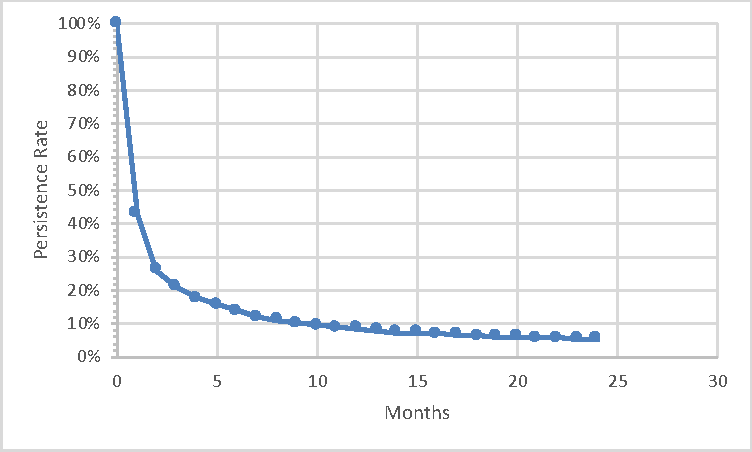
\includegraphics{figures/persistenceRateCrowdworks.pdf}
     \caption{Persistence Rate of Workers in CrowdWorks, according to the log of all workers who made accounts from January 1st, 2017 to December 31th, 2018.
     %\red{I hope this is okay to put in the paper. The figure needs to be improved. David: For the legend, maybe Persistence Rate of Workers on Crowdworks (50 workers, year 2019)? }
     }
     \label{fig:persistenceRate}
 \end{figure}

In December 2019, we conducted a poll of crowd workers on AMT and CrowdWorks, that have different characteristics; AMT is a microtask-based crowdsourcing platform, and CrowdWorks provides a wide variety of task types, focusing on a a bit larger tasks such as writing articles and codes.
This involved 101 workers (51 AMT and 50 CrowdWorks workers).
 Figure \ref{fig:surveyresult1}  summarizes the answers to the following questions: (Q1) Do you envision switching between platforms in the next X months? (Q2) How easy/challenging is switching between the platforms? 
 The result clearly shows that there is a strong correlation between worker mobility and the easiness of switching between platforms.
 We assume that since AMT is a pure microtask platform and obtaining a good reputation is easier, more workers think switching is easy in AMT than in CrowdWorks.
 Figure \ref{fig:surveyresult2} shows that workers would like platforms to have many advanced features that are not necessarily fully supported by the current generation of platforms. It is interesting to see that many workers on CrowdWorks dislike the collaboration feature among workers. We have not pursued the reasons yet, but a possible cause is the difference in the granularity of tasks. 

\begin{figure}[t]
\centering
\begin{tabular}{|c|c|c|c|c|c|c|c|}
\hline
Q1&Platform&\multicolumn{5}{|c|}{Q2}&Total\\
\cline{3-7}
&&Very Easy & Easy& Neither & Difficult & Very Difficult&\\
\hline
Yes&AMT&14\%&47\%&12\%&0\%&0\%&73\%\\
&CrowdWorks&0\%&2\%&6\%&2\%&0\%&10\%\\
\hline
No&AMT&4\%&6\%&6\%&10\%&2\%&26\%\\
&CrowdWorks&6\%&18\%&48\%&16\%&2\%&90\%\\
\hline
\end{tabular}
\caption{Results of Questions 1 and 2. The result suggests a correlation between the worker mobility  and the easiness of switching among crowdsourcing platforms.}
\label{fig:surveyresult1}
\end{figure}

\begin{figure}
    \centering
\begin{tabular}{|l|c|c|c|c|}
\hline
Q3. Preference for the feature?&Platform&\multicolumn{3}{|c|}{Answers}\\
\cline{3-5}
&&Like&Dislike&I don't know\\
\hline
Displaying Credentials&AMT&90\%&4\%&6\%\\
\cline{2-5}
&CrowdWorks&62\%&20\%&18\%\\
\hline
Specifying/ Quantifying/ Learning Skills&AMT&86\%&6\%&8\%\\
\cline{2-5}
&CrowdWorks&68\%&18\%&14\%\\
\hline
Anonymity&AMT&75\%&18\%&10\%\\
\cline{2-5}
&CrowdWorks&66\%&18\%&16\%\\
\hline
Complex Workflows&AMT&67\%&20\%&14\%\\
\cline{2-5}
&CrowdWorks&42\%&12\%&46\%\\
\hline
Collaboration&AMT&84\%&4\%&12\%\\
\cline{2-5}
&CrowdWorks&28\%&42\%&30\%\\
\hline
\end{tabular}
    \caption{Whether workers would like platforms to support for the features or not}
    \label{fig:surveyresult2}
\end{figure}

%\red{TBD after we get the poll results.}

\section{Platform Design}
\label{sec:platformDesign}

Based on the analysis of the poll of crowd workers
and extensive discussions with participants of the 2019 Shonan Seminar on Future of Work\footnote{ACM Sigmod Blog, Sept. 23, 2019,  \url{http://wp.sigmod.org/?p=2931}},
we have identified platform design as one of the key drivers
for ensuring the continued success of online job platforms.
We first identify a number of issues with the current platform design and make a number of concrete suggestions.

\textbf{Lack of Interoperability:}
The current generation of online job platforms operates in silos.
Even platforms that are in a specific domain such as driving (Uber, Lyft, Ola, Didi, etc.) are not
interoperable with each other.
A driver who has driven more than 10K rides with 4.9 rating in Uber will start
as a newbie when moving to a different platform such as Lyft.
This is also a problem for requesters. Consider a task that requires 10 experts.
It is possible that the labor market has the requisite experts -- but they are scattered across multiple platforms.
In this case, the requester could not successfully complete the task.
By enabling interoperability between platforms such issues and many more could be ameliorated.

\textbf{Lack of Support for Complex Tasks and Workflows:}
Currently, there are a limited number of tasks for which crowdsourcing is possible.
Even sophisticated platforms such as CrowdWorks only support as little as 200 types of tasks.
As more and more task types are being serviced by gig economy,
the need for supporting more complex tasks becomes important.
These complex tasks often have very different set of requirements.
For example, they might require a sophisticated workflow so that output of one stage is passed to another. They could require workers with different types of roles.
There might also be a need for specialized requirements such as splitting
a complex task into multiple sub-tasks that could then be assigned using a workflow.


\textbf{Limited Pricing Model:}
There are four types of pricing  models that are widely prevalent in online job platforms.
First is the fixed income model where each worker is given a fixed amount of money every month or so.
There is also task based pricing where the worker is paid a pre-agreed amount after completing a task.
There are some intermediate approaches such as fixed income plus a bonus amount and discounted pricing for completing large number of tasks.
Finally, there are competitions pricing  models in which we pay to the winner.
For online job platforms to thrive, it is important to have a wider variety of pricing models.

For the remainder of the section, we propose a number of improvements to platforms
that could either reduce the pain points of the key stakeholders or improve their satisfaction.

\subsection{Platform Design for Workers}
Workers are the back bone of a job platform by completing the tasks of requesters.
As discussed in the previous section, the current generation of platforms are not very conducive for
long term employment.

\textbf{Ease of On- and Off-boarding:}
One of the positive things about online job platforms is the flexibility they provide to the worker.
The worker can take tasks that are of interest to them while operating flexible hours.
Many platforms simplify them with as little as some identity document and bank account.
While joining the platform is straightforward, the onboarding process often leaves much to be desired.
Once the worker joins the platform, they are not provided enough guidance to contribute productively.
The worker is expected to learn how to contribute on their own.
Similar to offline employment in a traditional organization, it is important to have a proper onboarding procedure.
The current process for off-boarding is also ad-hoc.
Typically, workers and requesters can easily stop working in a platform.
However, the workers often lose the reputation that they have earned when moving to a different platform.
Similarly, the requesters also lose access to valuable and productive employees when moving to a different platform.
It is important to have a better off-boarding platforms so that the workers could transfer the reputation and knowledge learned from one platform to another.

\textbf{Support for Learning Skills.}
When a worker joins a platform, she often learns ``on-the-job''.
If the worker does not perform well due to inexperience, the job could be rejected by the requester
thereby affecting the approval rate of the worker.
Since a number of requesters filter workers based on task approval rate,
this could limit the number of tasks a new worker could contribute to.
This often leads to frustration of new workers and eventual turnover.
It is often desirable to have a more formal mechanism for simplifying this process.
For example, job platforms could have a collection of previously completed tasks
that could serve as an on-ramp for the workers.
By working on such tasks, the worker can learn the requisite skill in a low stress environment.


\textbf{Knowledge Base (KB) for Workers:}
Currently, there are a number of knowledge repositories in an
enterprise so that employees know the practices of the company.
It is important that online job platforms provide something similar.
Note that this is in addition to the aforementioned set of completed tasks.
As workers finish tasks, they must be able to add things to a personalized knowledge base
about what they learned from the task.
This could be public so that any worker can learn from it or
private where it is visible only to the worker.
As workers become increasingly knowledgeable, this serves as a repository for what they learned over the years.
Of course, this must also be interoperable and associated with the worker and transferable as needed.
This will also allow workers to find other mentors or experts to learn from.

%\scream{I moved Support of AI worker to the next session and added the following paragraph.}

\textbf{Support for Expressing Workers' Preference on Task Assignment}
The task assignment is usually done by workers themselves, partly because automatic assignment of  tasks to workers is not straightforward. There are many reasons for the worker to do the tasks; they did the task because it was easy to do, the task was interesting, they wanted to learn something from the task,  it gave them a lot of money, or it was the regular time slot for the worker to do tasks. If the platform has  the support for them to express their preferences, platforms will be able to automatically suggest them the tasks more accurately.






\subsection{Platform Design for Requesters}
In this subsection, we highlight some of the major pain points of requesters
and how new functionality from platforms could improve their satisfaction.

\textbf{Expressive Specification of Task Requirements.}
Currently, there is limited support from online job platforms for requesters
to precisely specify their requirements.
For example, in AMT, the requester can filter workers based on approval rate but cannot impose additional sophisticated filtering.
It is important for requesters to be able to specify worker requirements such as skills~\cite{DBLP:conf/www/MavridisGM16},
output requirements such as latency, cost and quality.
Furthermore, the requester could be open to various tradeoffs such as cost vs quality / latency.
For example, one might be willing to pay higher for better quality or faster response.
Unfortunately, current platforms do not provide such flexibility.

\textbf{Supporting Complex Tasks and Workflows.}
Almost all of the current job platforms support simple microtasks.
As more and more tasks are disrupted by the gig economy, it is important to have platforms that can support more complex tasks.
Often, complex tasks have a number of distinct requirements.
They are often knowledge intensive and collaborative~\cite{rahman2015task} requiring co-ordination with multiple workers.
They often are not monolithic and must be split into multiple sub-tasks
with different groups of workers completing each of them.
They also often require workers to embrace different roles.
Finally, they often have a complex workflow where the output of one stage is passed to the next.

\textbf{Support for Workflow Evolution and Changes during the Execution.} Workflows sometimes
need to change or evolve during the execution, since completing all tasks requires a long time in
general and it is often the case that we find better workflows after we start to execute the
original workflow. The platforms should support this kind of evolution and changes of workflows
with a minimum amount of effort.

\textbf{Sophisticated Algorithms for Assigning Workers to Tasks.}
Currently, most crowdsourcing platforms do not have
any sophisticated algorithms in matching workers to tasks.
Often, this is done manually by the workers by browsing the list of available tasks.
Other than filtering the pool of workers, requesters do not have much control on which workers perform the tasks.
Despite extensive research in algorithms for task assignment~\cite{basu2015task,ho2012online,rahman2015task},
they are not often incorporated into the platforms.
It is important to either have sophisticated algorithms for task assignment so that requester specifications are satisfied or provide an alternate way for the requesters to select workers.

\textbf{Support for AI Workers.}
Given the increasing capabilities of AI, it is a matter of time when AI workers become a major part of online job platforms.
There are a number of scenarios where AI workers could be useful.
If there are urgent tasks, then it is not always possible to use humans to answer them.
Often, there is a substantial latency when humans are involved.
In these circumstances, AI workers could be a valuable resource.
Alternatively, the requester could be cash-strapped and willing to accept less
accurate results in exchange for cheaper payments.
There are many collaborative situations where AI takes care of the boring work
while the human works on the subset that requires human intuition.
Finally, AI and humans should be able to replace each other in some situations: an AI
can be used as a fallback is a human is answering too late to an urgent task, and
conversely, humans can be used as a fallback if an AI fails at recognizing something critical.
However, one must be careful in how AI workers are integrated.
If not, they could replace human workers causing significant social strife.
Furthermore, it is important for requesters to understand the advantages and limitations of the AI workers.


\textbf{Total Optimization.}
Currently, most of the work on matching is done in a piecemeal manner
where best workers are identified for each task.
It is often important to have a holistic optimization
that takes the preferences of all the stakeholders into account.
This would ensure that good workers are overloaded with work
and the workers/tasks are matched in a fair manner. 

\textbf{Algorithm Boutiques:}
A typical crowdsourcing platform could be improved by incorporating algorithms into the major components including (i) how the task requirements are specified (ii) how tasks are assigned to workers (iii) how the ground truth of tasks are obtained by aggregating worker responses and (iv) how the skills of workers are learned based on their response to tasks.
Unfortunately, most of the platforms do not incorporate any of these algorithms.
Most of these points are offloaded to the workers and requesters.
While experienced requesters often have a concrete mechanisms to effectively achieve each of them,
the vast majority of requesters have an ad-hoc and sub-optimal procedure.
Finally, even if some platforms implement the algorithms, they are often opaque
and the requesters have no say in how they are chosen.
It is important for a crowdsourcing platform to have a boutique of algorithms
from which requesters can choose the specific variants.

\textbf{Bespoke Platforms:}
Most of the crowdsourcing platforms are not very customizable.
For example, a domain scientist might need a custom crowdsourcing platform for the task at hand.
Currently, the scientist is left with two unappealing choices.
Either use an existing platform by approximating the task to suit the constraints of the platform.
Alternatively, the scientist could build a new platform from scratch at tremendous cost.
In order to unleash the future of work, it is important to enable any requester
to create custom online job platforms.
It must have a set of default algorithms that could be customized by the requester.
The emergence of on-demand computing frameworks such as Amazon AWS or Microsoft Azure
lowered the cost of startups by relieving them of the pressure of managing servers.
We believe that the time is ripe to do something analogous for crowdsourcing.

\textbf{Library of Workflows and AI Workers.}
In order to help new requesters, it is important for crowdsourcing platforms to provide a large collection of commonly used workflows.
Similarly, they could also provide some AI workers that could perform limited set of tasks
albeit with the understanding that the work could be of lower quality that of a human.

\textbf{Open Source Academic Platforms.}
Most of the online job platforms are closed source and proprietary. 
This inhibits research on improving various components of the platform and evaluate the potential impact.
One natural solution for driving further research in platform design is through open source academic platforms.
A well designed and modular platform could allow a researcher to modify certain components, investigate how it impacts the stakeholders 
and use to improve platform design.
Currently, the researcher has to more or less implement the end-to-end crowdsourcing platform which could be prohibitively challenging.
There are a number of promising options such as Headwork and Crowd4U. Headwork~\footnote{\url{http://headwork.gforge.inria.fr}} is a proof-of-concept crowdsourcing platform focusing on skill modeling and complex task workflows, using Tuple Artifacts. Crowd4U~\cite{morishima2014crowd4u} is a nonprofit open microvolunteering and crowdsourcing platform for academic and public purposes.
It has been widely used for tasks such as identifying building damages during natural disasters, annotative tweets, translation,
identifying paths of tornados and so on. 
The most appealing property is its ability to extend the functionality through a datalog type language called CyLog~\cite{morishima2012cylog}.
For example, when the authors came up with an algorithm~\cite{rahman2015task} for task assignment in collaborative crowdsourcing setting
they were able to easily implement it on top of Crowd4U~\cite{ikeda2016collaborative}.
Such functionality has the potential to dramatically improve crowdsourcing research on platform design. 

\section{Platform Interoperability}
\label{sec:platformInteroperability}


\begin{figure*}
\small
\begin{tabular}{|p{15mm}|p{3cm}|p{15mm}|p{15mm}|p{15mm}|p{15mm}|p{15mm}|p{15mm}|}
\hline
&&\multicolumn{6}{|l|}{Platforms for$\ldots$}\\
\cline{3-8}
Support for$\ldots$&Functionalities&Providing Jobs&Worker Communication&Worker/ Requester Profiles& Task-Worker Matching&Workflow
management&Worker Training\\
\hline
Worker&Ease of On- and off-boarding&$\bigcirc$&&$\bigcirc$&&&\\
\cline{2-8}
&Learning Skills&&$\bigcirc$&&&&$\bigcirc$\\
\cline{2-8}
&KB for workers&&&&&$\bigcirc$&\\
\cline{2-8}
&Worker Preference Specification&$\bigcirc$&&$\bigcirc$&&&\\
\cline{2-8}
&Ease of choosing tasks&$\bigcirc$&$\bigcirc$&$\bigcirc$&$\bigcirc$&&\\
\hline
Requester&Task Requirement Specification&$\bigcirc$&&&&&\\
\cline{2-8}
&Complex Workflow&&&&&$\bigcirc$&\\
\cline{2-8}
&Sophisticated Assignment Algorithm&&&&$\bigcirc$&$\bigcirc$&\\
\cline{2-8}
&AI Worker Support&&&$\bigcirc$&$\bigcirc$&$\bigcirc$&\\
\cline{2-8}
&Total Optimization&&&&&$\bigcirc$&$\bigcirc$\\
\cline{2-8}
&Algorithm Butiques&&&&$\bigcirc$&$\bigcirc$&\\
\cline{2-8}
&Total Optimization&&&&&$\bigcirc$&$\bigcirc$\\
\cline{2-8}
&Bespoke Platforms&$\bigcirc$&&$\bigcirc$&&&$\bigcirc$\\
\cline{2-8}
&Workflow and AI Worker Library&&&$\bigcirc$&&$\bigcirc$&\\
\hline
\end{tabular}
\caption{Relationship between functionalities and platforms for FoW. 
This suggests that cooperation between different platforms will be the key to make use of the full potential of ecosystem of FoW platforms. 
%The circle/triangle can be replaced with terms that explain what is provided by the platform.
}
\label{fig:functionsandplatforms}
\end{figure*}

In the previous section, we discussed the various functionalities that could be added to the platform to improve it.
In this section, we discuss how additional benefits could be obtained by enabling interoperability between platforms.
A vast ecosystem has emerged around online job platforms.
We begin by creating a taxonomy of such platforms and discuss how these functionalities could be improved and integrated.


\subsection{Taxonomy of Online Job Platforms and Ecosystems}





So far, the prior work has extensively discussed online job platforms such as AMT or CrowdWorks.
However, there is a thriving ecosystem built around these platforms.
They often add features missing in the original platforms or provide value added services.
In order to improve platform design, it is important to understand this ecosystem.


\textbf{Job Platforms.}
For the sake of completeness, we include online job platforms in the taxonomy.
These are the platforms such as AMT, CrowdWorks and others where requesters post tasks
and workers complete them \emph{online}.
These could be generic platforms where a wide variety of tasks are performed or
specific ones such as ride-hailing that perform a single task.

\textbf{Platforms for Worker Communication.}
Most of the current platforms do not support communications between workers.
Some times, this is desirable to avoid inter-worker collusion.
Most of the time, this is very limiting as collaborative tasks become more and more important.
Furthermore, there are also many scenarios where workers might want to communicate.
These include providing feedback about requesters, providing tips and so on.
So there is an emerging set of platforms to enable such communication.
The most popular of these are Turkopticon~\cite{irani2013turkopticon} and TurkerNation (which closed in 2018).
Turkopticon has almost 500K reviews of around 50K requesters.
It also provides granular way to provide requestor feedback on fairness, pay quality and speed of payment.
While these are a good start, both Turkopticon and TurkerNation were specific to AMT.
It is important that most of these platforms provide a mechanism for worker communication.
This could be done within each platform or by providing a generic website where workers from different platforms can congregate.

\textbf{Platforms for Persistent Worker/Requester Profiles.}
Currently, each online job platform has an internal mechanism for measuring worker/requestor reputation.
This could be as simple as approval rate for workers and requesters.
It could also be more granular such as how many tasks a worker has completed for each skill.
It is important to have persistent profiles for both workers and requesters so that
they can build their reputations based on their entire body of work.
Currently, if an experienced worker moves from one platform to another,
she has to start from scratch.
Hence, it is important to have an independent website where workers/requesters
can create a profile and share all relevant information in a verified manner.

\textbf{Platforms for Matching Workers and requesters.}
The explosion of online job platforms makes it harder for both workers and requesters.
Productive workers and fair requesters are often scattered across platforms.
Each worker has to login to multiple platforms to find useful work that quickly becomes tedious.
It is desirable to have platforms that could match workers and requesters across multiple platforms.
For example, the worker could specify task preferences and the matching platform will scour
other online job platforms and notify the worker when relevant tasks become available.
This could also benefit requesters by finding productive workers across platforms.
While there are some preliminary effort such as by CrowdWorks or Figure Eight
that act as a layer on top on AMT, there is still lot of work to be done.

\textbf{Towards Better and Fairer Crowdsourcing Platforms.}
Recently, there has been increasing interest in improving crowdsourcing.
Some of these efforts include providing guidelines for requesters for specific platforms.
Popular examples include Dynamo Guidelines~\cite{salehi2015we} for academic requesters and FairCrowdWork.org.
These often help well-meaning requesters to treat workers properly
by providing clear instructions about the task and fair pay.
FairCrowdWork.org provides advice to workers based on their rights.
They have extensive survey involving 95 questions that allows workers to rate various crowdsourcing platforms.
Specifically, they quizzed workers on 8 topics including demographics, work experience in a platform, payment details, communication with requesters and platforms, reliability of the platform, quality of available tasks and miscellaneous information.
Based on the response of the workers, each platform is graded in a scale between 1-5.




\subsection{Platform Interoperability}
Given the plethora of platforms, it is important they are interoperable to ensure that
workers and requesters have a wide variety of options.
Currently, interoperability is nearly non-existent.
However, we believe that this will become more and more important
as an increasing proportion of workers join these online job platforms.

There are a number of dimensions in which interoperability must be achieved.
Workers should be able to move between platforms without losing any of their skills/ratings etc.
This will require the creation of a unified schema of skills. This could be different for each domain.
Once this is done, each platform has to fill the worker skills according to this schema.
Of course, each platform could have their own additional proprietary list of metric.
Nevertheless, it must be possible to create a worker ``profile'' that gives a holistic
perspective of the worker skills in that domain regardless of how many platforms the
worker is involved with.
Interoperability must also be possible from a requestor perspective. Given a task, it must be
possible to recruit workers from multiple platforms.
For example, if a requestor needs 10 qualified experts, it must be possible to
recruit 4 from Platform 1, 5 from Platform 2 and 1 from a third one.
Similarly, it is important to create a requester ``profile'' that is persistent across multiple platforms
so that the worker has a holistic perspective of the requester such as the rate of rejection of tasks. 

We can see that achieving interoperability is quite challenging.
This requires a commonly agreed standard of skills, which,
due to the richness and specialties of the many disciplines that
exist, is probably difficult to achieve.
For platforms to exchange information, one must design a common, unifying API
that will fit for all types of applications.

\textbf{Standardized API and Schema:} 
The diversity of the crowdsourcing and FoW platforms makes standardization much challenging.
However, it is possible that specific components such as task creation, worker selection, truth inference, worker skill estimation
could be more amenable for standardization.
The creation of the standard API would boost the adoption of crowdsourcing by bringing in more enterprises.
Entrepreneurs could also create innovating applications for specific crowdsourcing tasks.
This is akin to the explosion of smartphone apps once iOS and Android provided a standardized API functionality.
For example, one could identify an important tasks such as Entity Resolution (finding tuples that represent the same real-world entity)
and use the API of the platforms to recruit the crowd, perform the tasks and provide the results. 
There will also be standardization in terms of how metadata about workers and tasks are stored \cite{DBLP:books/daglib/0031391,DBLP:journals/www/SchallSP14}.

\textbf{Interchange Format:} There is a need to have a pre-defined interfaces and Schema for data
exchanges between platforms. It should provide a simple agreed model that has enough
expressive power to achieve total optimization. 
At the minimum, one must be able to transfer the human factors of workers (such as skill, past tasks, etc)
and that requesters (task approval rate, etc). 
This allows both these types of users to migrate to a different platform without being locked in. 

\textbf{Interchange Queries:} When data is not large and is allowed to be exported, platforms can exchange the whole data in the interchange format,
but there are cases where this is not a practical solution. An effective approach is to  develop common sets of interchange queries so that we can identify only small subsets of data to be exchanged.




\section{Conclusion}
With these two simple innovations, we can move past the conflicts and controversy and on to utilizing privacy-sensitive mobile contact tracing to improve the efficacy of public health measures - thereby saving lives and unnecessary suffering - while respecting civil liberty.  The companies should provide the interoperable building blocks without themselves getting into the business of providing the Apps or holding the data.  They can maintain their privacy-first, decentralization posture, but should advocate for an interoperable COVID key Commons, rather than dictating policy on the app ecosystem.  Government actors can regain policy determination and influence the app ecosystem so as to best tailor offerings to their constituents. The tailoring could include questions around how best to provide a Commons of appropriate scale, and utilize physical measures to relate anonymous key reports to the places within their jurisdiction. Government actors already have extensive experience with civic infrastructure such as security cameras, traffic signals and health inspections. They can apply the similar principles towards recognizing the importance of public awareness, potential for creating stigma, and bringing benefit to non-participating members of the communities.  The technology can assist the contact tracing process, but should not be dictating it or replacing the human relationship of the patient and the health professionals performing interviews and care.  The trust that is built there is what makes opt-in approaches viable, and only with appropriate individual protections.
\vspace{-.6cm}
\enlargethispage{1cm}
\bibliographystyle{abbrv}

\begin{thebibliography}{10}

\bibitem{basu2015task}
S.~Basu~Roy, I.~Lykourentzou, S.~Thirumuruganathan, S.~Amer-Yahia, and G.~Das.
\newblock Task assignment optimization in knowledge-intensive crowdsourcing.
\newblock {\em The VLDB Journal—The International Journal on Very Large Data
	Bases}, 24(4):467--491, 2015.

\bibitem{brawley2016work}
A.~M. Brawley and C.~L. Pury.
\newblock Work experiences on mturk: Job satisfaction, turnover, and
information sharing.
\newblock {\em Computers in Human Behavior}, 54:531--546, 2016.

\bibitem{doan2011crowdsourcing}
A.~Doan, R.~Ramakrishnan, and A.~Y. Halevy.
\newblock Crowdsourcing systems on the world-wide web.
\newblock {\em Communications of the ACM}, 54(4):86--96, 2011.

\bibitem{ho2012online}
C.-J. Ho and J.~W. Vaughan.
\newblock Online task assignment in crowdsourcing markets.
\newblock In {\em Twenty-Sixth AAAI Conference on Artificial Intelligence},
2012.

\bibitem{ikeda2016collaborative}
K.~Ikeda, A.~Morishima, H.~Rahman, S.~B. Roy, S.~Thirumuruganathan,
S.~Amer-Yahia, and G.~Das.
\newblock Collaborative crowdsourcing with crowd4u.
\newblock {\em Proceedings of the VLDB Endowment}, 9(13):1497--1500, 2016.

\bibitem{irani2013turkopticon}
L.~C. Irani and M.~Silberman.
\newblock Turkopticon: Interrupting worker invisibility in amazon mechanical
turk.
\newblock In {\em Proceedings of the SIGCHI conference on human factors in
	computing systems}, pages 611--620. ACM, 2013.

\bibitem{DBLP:conf/www/MavridisGM16}
P.~Mavridis, D.~Gross{-}Amblard, and Z.~Mikl{\'{o}}s.
\newblock Using hierarchical skills for optimized task assignment in
knowledge-intensive crowdsourcing.
\newblock In {\em Proceedings of the 25th International Conference on World
	Wide Web, {WWW} 2016, Montreal, Canada, April 11 - 15, 2016}, pages 843--853,
2016.

\bibitem{mcfeely2018workplace}
S.~McFeely and R.~Pendell.
\newblock What workplace leaders can learn from the real gig economy. gallup,
2018.

\bibitem{morishima2014crowd4u}
A.~Morishima, S.~Amer-Yahia, and S.~B. Roy.
\newblock Crowd4u: An initiative for constructing an open academic
crowdsourcing network.
\newblock In {\em Second AAAI conference on human computation and
	crowdsourcing}, 2014.

\bibitem{morishima2012cylog}
A.~Morishima, N.~Shinagawa, T.~Mitsuishi, H.~Aoki, and S.~Fukusumi.
\newblock Cylog/crowd4u: A declarative platform for complex data-centric
crowdsourcing.
\newblock {\em Proceedings of the VLDB Endowment}, 5(12):1918--1921, 2012.

\bibitem{rahman2015task}
H.~Rahman, S.~B. Roy, S.~Thirumuruganathan, S.~Amer-Yahia, and G.~Das.
\newblock Task assignment optimization in collaborative crowdsourcing.
\newblock In {\em 2015 IEEE International Conference on Data Mining}, pages
949--954. IEEE, 2015.

\bibitem{salehi2015we}
N.~Salehi, L.~C. Irani, M.~S. Bernstein, A.~Alkhatib, E.~Ogbe, K.~Milland,
et~al.
\newblock We are dynamo: Overcoming stalling and friction in collective action
for crowd workers.
\newblock In {\em Proceedings of the 33rd annual ACM conference on human
	factors in computing systems}, pages 1621--1630. ACM, 2015.

\bibitem{DBLP:books/daglib/0031391}
D.~Schall.
\newblock {\em Service-Oriented Crowdsourcing - Architecture, Protocols and
	Algorithms}.
\newblock Springer Briefs in Computer Science. Springer, 2012.

\bibitem{DBLP:journals/www/SchallSP14}
D.~Schall, B.~Satzger, and H.~Psaier.
\newblock Crowdsourcing tasks to social networks in bpel4people.
\newblock {\em World Wide Web}, 17(1):1--32, 2014.

\end{thebibliography}

\end{document}
